% Decryption of one ciphertext: submit, optional reveal (locked applications only),
% threshold partials, combine. Every arrow into the contract is a transaction.
\begin{figure}[t]
\centering
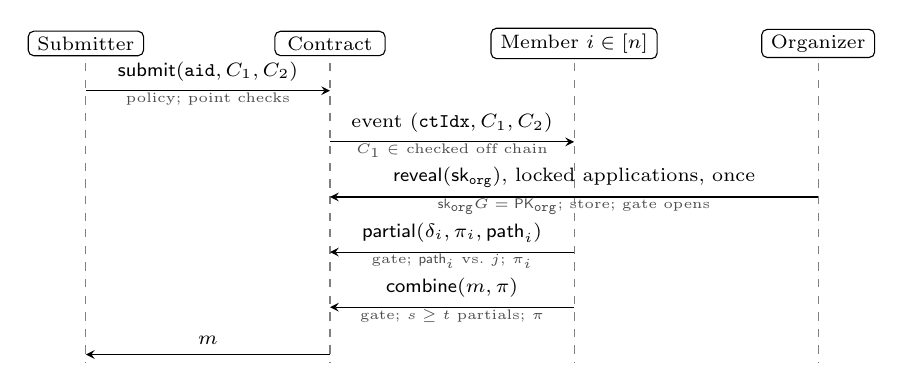
\begin{tikzpicture}[font=\scriptsize, >=stealth, note/.style={inner sep=0.5pt, font=\tiny, text=black!70}]
  \def\colS{0} \def\colC{3.1} \def\colM{6.2} \def\colO{9.3}
  \foreach \x/\n in {\colS/Submitter, \colC/Contract, \colM/Member $i \in [n]$, \colO/Organizer} {
    \node[draw, rounded corners=2pt, minimum width=1.4cm, inner ysep=2pt] at (\x,0) {\n};
    \draw[dashed, gray] (\x,-0.25) -- (\x,-4.05);
  }
  \draw[->] (\colS,-0.6) -- node[above] {$\mathsf{submit}(\mathtt{aid}, C_1, C_2)$}
    node[below, note] {policy; point checks} (\colC,-0.6);
  \draw[->] (\colC,-1.25) -- node[above] {event $(\mathtt{ctIdx}, C_1, C_2)$}
    node[below, note] {$C_1 \in \GC$ checked off chain} (\colM,-1.25);
  \draw[->] (\colO,-1.95) -- node[above] {$\mathsf{reveal}(\mathsf{sk}_{\mathtt{org}})$, locked applications, once}
    node[below, note] {$\mathsf{sk}_{\mathtt{org}} G = \mathsf{PK}_{\mathtt{org}}$; store; gate opens} (\colC,-1.95);
  \draw[->] (\colM,-2.65) -- node[above] {$\mathsf{partial}(\delta_i, \pi_i, \mathsf{path}_i)$}
    node[below, note] {gate; $\mathsf{path}_i$ vs.\ $\mroot{j}$; $\pi_i$} (\colC,-2.65);
  \draw[->] (\colM,-3.35) -- node[above] {$\mathsf{combine}(m, \pi)$}
    node[below, note] {gate; $s \ge t$ partials; $\pi$} (\colC,-3.35);
  \draw[->] (\colC,-3.95) -- node[above] {$m$} (\colS,-3.95);
\end{tikzpicture}
\caption{Decryption of a ciphertext on pool key $P_j$; arrows into the contract are transactions. Partials and the combine carry Groth16 proofs, partials also a Merkle path for $D_{j,i}$; the gate is the decryption window plus, for locked applications, the one-shot reveal.}
\label{fig:decryption}
\end{figure}
